\chapter{Principe de la solution envisagée}
\label{chap:sol}

  Notre solution est découpée en trois étapes incrémentales. Dans un premier
  temps, nous allons rétablir le procédé de migration de processus
  mono-thread. Dans un second temps, nous ajouterons le support du
  multi-thread. Enfin, nous allons ré-implémenter un composant d'ALMOS appelé
  DQDT, responsable de la politique de migration dans le noyau.

  \begin{paragraph}{Remarque:}
    Dans la section~\ref{sec:mono}, le mot \textit{processus} est utilisé pour
    désigner un processus composé d'un seul thread. Dans la suite de ce
    chapitre, et notamment en section~\ref{sec:multi}, on considère des
    processus avec plusieurs threads.
  \end{paragraph}


  \section{Support des processus mono-thread}
  \label{sec:mono}

    Cette première étape à pour but de mettre en place deux mécanismes:
    \benumline \item la création distante de processus et \item la migration de
    processus entre noyaux\eenumline. Pour compléter ces deux objectifs, il est
    nécessaire de définir l'ensemble des structures partagées par les processus,
    lesquelles devront nécessairement être maintenues cohérentes tout au long de
    l'exécution.

    \subsection{Principes}

      \subsubsection{Création distante}
        Ce mécanisme permet au noyuau de créer le processus résultat d'un
        \texttt{fork()} sur un autre noyau que lui-même. Pour cela, on va se
        baser sur l'appel système \texttt{exec()}. Ce dernier, utiliser de pair
        avec \texttt{fork()}, permet de remplacer totalement le programme
        exécuté par le processus appelant.

        Lors d'un \texttt{fork()}, un nouveau processus, copie du père, sera
        créé. Celui-ci restera sur le même c\oe ur que son père jusqu'à son
        appel à \texttt{exec()}. Un exemple d'utilisation de ces deux fonctions
        est donné ci-dessous.
        \clearpage

        \lstinputlisting[ caption=Utilisation de
          \texttt{fork-exec}]{include/code/example.c}
        \FloatBarrier

      Attendre un appel à \texttt{exec()} pour effectuer la \textit{vraie}
      création permet de ne pas briser la localité spatiale des processus
      parents, qui par définition accèdent aux mêmes données.\\

      Cet appel système sera donc modifié en ajoutant le mécanisme de migration,
      qui repose entièrement sur les RPC du noyau. Lors de la migration, le
      noyau source enverra par passage de message au noyau destinataire toutes
      les informations nécessaires pour reconstruire l'espace d'adressage
      virtuel du nouveau processus.

      \begin{paragraph}{Remarque:}
        Un appel à \texttt{exec()} ne migrera pas toujours un processus. La
        migration se fera selon différents paramètres fourni par la DQDT.
      \end{paragraph}

      \subsubsection{Migration}

        Sur le même principe que le création distante, la migration repose sur
        le mécanisme des RPC du noyau. La seule différence est le fait de
        pouvoir migrer un processus entier en dehors de l'appel système
        \texttt{exec()}. Cette opération est uniquement envisagée pour préparer
        l'ajout du support multi-thread.


    \subsection{Maintien de cohérence}

      Comme nous l'avons vu précédemment, ces deux opérations représentent un
      enjeux quant aux structures de données que contiennent les processus, et
      surtout celle qu'ils partagent. Nous avons identifié les structures
      suivantes comme étant problématiques dans notre cas:
      \begin{itemize}
      \item les descripteurs de fichiers
      \item les zones mémoires
      \end{itemize}
      \begin{paragraph}{Remarque:}
        Tous les processus n'ont pas de zones mémoire partagées avec d'autres.\\
      \end{paragraph}

      Afin de faciliter le maintien de la cohérence lors d'une migration, nous
      allons redéfinir le fonctionnement des descripteurs de fichiers et des
      zones mémoires. Il est nécessaire de s'abstraire de l'utilisation des
      pointeurs qui deviennent inutiles lorsqu'un processus change de noyau. En
      effet, une adresse virtuelle dans un noyau $N$ n'est pas toujours
      significative dans un noyau $N'$. Un bon exemple pour illustrer notre cas
      est celui des processus parents/enfants. Chaque processus doit savoir qui
      est son père, et possède un pointeur en direction de la \texttt{struct
        task} de ce père. Si le fils est migré sur un nouveau noyau, cette
      adresse est devenue obsolète.

      Nous allons donc réduire au maximum le nombre de pointeurs, et notamment
      ceux utilisés pour gérer les descripteurs de fichiers ouverts ainsi que
      les zones de mémoire virtuelle d'un processus.  Supprimer ces pointeurs
      implique de devoir changer la structure de données utilisée pour stocker
      toutes les informations. Nous allons utiliser des tableaux pour
      enregistrer les informations sur les fichiers ouverts par les
      processus. Ces tableaux seront plus faciles à migrer puisqu'ils s'agira
      seulement d'en faire une copie dans la mémoire du noyau destinataire.

      En ce qui concerne les régions virtuelles, nous avons actuellement deux
      solutions à l'étude et aucune n'a pour l'instant été choisie:
      \begin{itemize}
        \item utiliser une table de hash par calcul
          (figure~\ref{fig:calculated-hash-table})
        \item utiliser une table de hash chainée
          (figure~\ref{fig:hash-chained-table})
      \end{itemize}

      \begin{paragraph}{La table de hash par calcul:}

        \todo{}
        \begin{figure}[ht]
          \centering
          %% \includegraphics[scale=0.5]{calculated-hash-table}
          \caption{Une table de hash par calcul.}
          \label{fig:calculated-hash-table}
        \end{figure}

      \end{paragraph}


      \begin{paragraph}{La table de hash chainée:}

        \begin{figure}[ht]
          \centering
          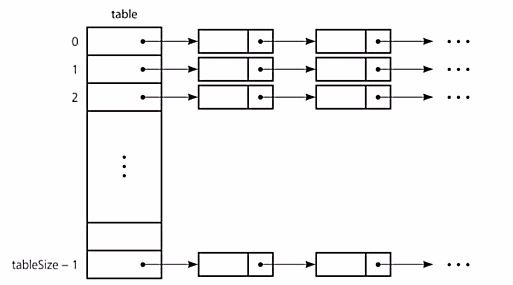
\includegraphics[scale=0.5]{hash-chained-table}
          \caption{Une table de hash chaînée. Chaque index contient un pointeur
            vers une liste chainée. Dans notre cas, on aura les structures
            représentant les régions virtuelles.}
          \label{fig:hash-chained-table}
        \end{figure}

        Comme on veut réduire le nombre de pointeurs, on ne va pas utiliser des
        listes chainées ``classiques''. En effet, les pointeurs \textit{next} ne
        pointeront pas vers le maillon suivant de la chaine, mais vers un
        tableau des différents PFN d'un processus. Ils transporteront également
        une valeur d'\textit{offset}. Grâce à ce PFN et cet offset, on pourra
        retrouver l'adresse physique du maillon correspondante. Une simple
        traduction vers une adresse virtuelle permet de retrouver ce maillon.

        Quelque soit la solution envisagée, les entrées et sorties sont
        similaires, ce qui nous permet de n'effectuer qu'une seule
        spécification. Nous allons utiliser l'adresse virtuelle accédée comme
        entré de la fonction de hash. En sortie, nous obtenons l'adresse
        physique correspondante.

        \begin{center}
          \texttt{hash(vaddr) = paddr}
        \end{center}

      \end{paragraph}

      La première solution nous garanti de n'avoir qu'une table à
      gérer. Néanmoins, cette gestion est assez difficile dans son
      implémentation. À l'inverse, la table de hash chainée est plus simple à
      mettre en \oe uvre mais elle offre une représentation visuelle plus
      complexe que la précédente solution. Ces deux solutions n'ont pour
      l'instant pas été estimées en terme de coût pour le système. Elles restent
      donc à l'état d'hypothèse jusqu'à ce que l'une d'elle s'avère plus
      efficace.

    %% \subsection{Les descripteurs de fichiers}

    %%   Les \textit{file descriptors} sont une abstraction des systèmes
    %%   d'exploitation permettant aux processus de manipuler des fichiers. Ce sont
    %%   en réalité des structures de données pointant sur une autre structure
    %%   appelée \texttt{struct file}. Celle-ci contient notamment la valeur de la
    %%   tête de lecture, appelé \textit{offset}, et un compteur de référence
    %%   permettant de savoir combien de \textit{file descriptors} pointent sur la
    %%   \texttt{struct file}, \textit{i.e,} combien de fois le fichier à été
    %%   ouvert.

    %%   Lors d'un \texttt{fork()}, un processus enfant héritera de certaines
    %%   informations de son père. La norme POSIX~\citep{posix2013} impose
    %%   notamment qu'un processus enfant doit avoir accès aux fichiers ouverts par
    %%   son père. Néanmoins, un fichier ouvert après un \texttt{fork()} n'est pas
    %%   partagé avec le processus père. Ces deux mécanismes sont illustrés par la
    %%   figure~\ref{fig:file-descriptors}. Le mécanismes des \texttt{inode} est
    %%   introduit juste après.

    %%   \begin{figure}[ht]
    %%     \centering
    %%     \includegraphics[scale=0.5]{file-descriptors-2}
    %%     \caption{Partage d'une \texttt{struct file}. Le processus $A$ appelle
    %%       \texttt{fork()} et crée le processus $C$. Ils partagent la même table
    %%       mais n'ont aucun fichier en commun. $A$ ouvre le fichier
    %%       \texttt{A\_Filename} puis fait un nouveau \texttt{fork()}, créant le
    %%       processus $B$. Ce dernier partage alors la \texttt{struct file}
    %%       pointée par son père.}
    %%     \label{fig:file-descriptors}
    %%   \end{figure}

    %%   Ce partage implique que la tête de lecture soit la même pour les deux
    %%   processus. Lors d'un \texttt{read()} ou d'un \texttt{write()} par le
    %%   processus $A$, celui-ci change la valeur de la tête de lecture. Ce
    %%   changement doit être visible par le processus $B$.

    %%   Cette obligation se révèle problématique dans le cas d'une migration. En
    %%   effet, si un processus enfant est changé de noyau, il est changé d'espace
    %%   d'adressage. Il ne peut donc plus accéder aux données de son père de
    %%   manière directe, et doit utiliser le passage de message. Cette opération
    %%   est très coûteuse, et est source de contention dans le cas des messages de
    %%   cohérence pour la modification de la tête de lecture.\\

    %%   Nous allons changer la gestion des compteurs de références et des
    %%   \textit{offset} du noyau ALMOS. Dans un premier temps, nous allons nous
    %%   abstraire des \textit{file descriptors}. Plutôt que d'avoir des pointeurs
    %%   sur les \texttt{struct file} des fichiers ouverts, nous allons placer au
    %%   sein des processus un tableau contenant ces structures. L'utilisation d'un
    %%   tableau permet de s'affranchir des pointeurs qui sont problématiques lors
    %%   des migrations.

    %%   Ensuite, nous allons changer l'emplacement de l'\textit{offset}. Nous
    %%   allons le déplacer au sein de la \texttt{struct inode}. Un \textit{inode}
    %%   est une structure de donnée représentant le fichier au sein du système de
    %%   fichier. Elle est pointée par les \texttt{struct file} et possède un
    %%   compteur de références fonctionnement sur le même modèle que vu
    %%   précédement.

    %%   \begin{paragraph}{Remarque:}
    %%     La différence entre une \texttt{struct inode} et une \texttt{struct
    %%       file} peut être expliquée comme suit. Soit deux fichiers, dont un est
    %%     un lien symbolique vers l'autre. Ces deux fichiers auront deux
    %%     \texttt{struct file} différentes, car un lien symbolique \textit{est} un
    %%     fichier. Néanmoins, il n'y a qu'un seul fichier \textit{réel} sur le
    %%     disque, qui est matérialisé par sa \texttt{struct inode}. Chaque
    %%     \textit{inode} est unique sur le système.\\
    %%   \end{paragraph}

    %%   Le fait de gérer l'offset d'un fichier directement dans l'\textit{inode}
    %%   nous assure par construction de la cohérence de la valeur de la tête de
    %%   lecture lors de tous les accès, quelque que soit la localisation du
    %%   processus effectuant l'opération. La migration d'un processus sera
    %%   d'autant plus facilitée puisqu'il suffira simplement de copier le tableau
    %%   des \texttt{struct file} du père, l'offset étant gérer dans
    %%   l'\textit{inode}.


    %% \subsection{Les zones mémoire}

  \section{Ajout du multi-thread}
  \label{sec:multi}  

    Une fois le support des processus mono-thread en place, nous allons ajouter
    le support du multi-thread. Cette opération s'avère très délicate, et
    représente probablement l'étape la plus compliquée de ce stage. De plus,
    malgré une étude du sujet, il est possible de découvrir de nouveaux
    problèmes au cours de notre avancée.\\

    Dans la section~\ref{sec:mono}, nous avons présenté les structures de
    données critiques dans le cas d'applications se basant sur des processus et
    non des threads. Nous allons à présent nous intéresser à ces derniers. Après
    étude du problème, nous avons considéré les structures suivantes comme
    problématiques lors que la migration de threads:
    \begin{itemize}
      \item la table des pages
      \item les signaux
    \end{itemize}  

    \subsection{La table des pages}

      La table des pages est la structure de données des processus permettant
      d'effectuer les traductions d'adresses. Chaque processus possède sa propre
      table des pages. Tous les threads d'un processus accèdent de manière
      atomique à cette table lorsqu'ils veulent ajouter de nouvelle pages. Le
      problème de cette strucutre est sa granularité de partage: on considère un
      processus entier comme propriétaire. Si l'on migre un thread du processus
      sur un autre noyau, ce dernier devra faire des accès par passage de
      messages sur la table, ce qui n'est pas envisageable pour des raisons de
      performances. Il faut donc copier la table des pages entièrement, ce qui
      n'est pas gratuit, et maintenir ensuite une cohérence entre toutes les
      tables répliquées dans les clusters. En prenant en compte le fait que
      chaque processus possède une table de page, les surcoûts liés aux
      communications apparaîssent rapidement.

      Pour répondre à cette problématique, nous allons intégrer une nouvelle
      granularité pour la table des pages. En effet, nous allons affectuer une
      table des pages par thread et non par processus. Cette table contiendra
      certaines pages communes avec les autres threads du processus, mais aura
      également ses propres pages. Le mécanisme proposé est illustré par la
      figure~\ref{fig:almos-page-table}.

      \begin{figure}[ht]
        \centering
        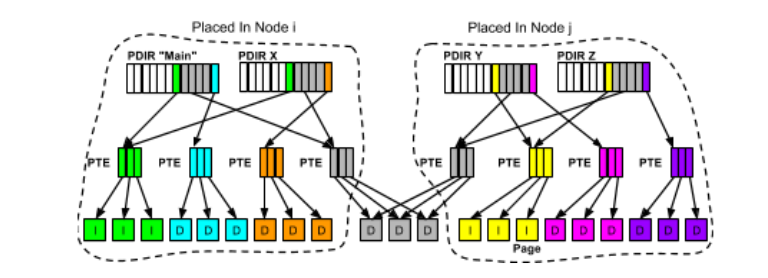
\includegraphics[width=\textwidth]{almos-page-table}
        \caption{Organisation de la table des pages pour quatre threads d'un
          même processus. Deux threads sont placés sur un cluster $I$, et deux
          sur un cluster $J$. Les threads partagent certaines pages de données
          et d'instruction, parfois entre clusters, mais ont également leur
          pages privées~\citep{almaless2014universite}.}
        \label{fig:almos-page-table}
      \end{figure}

      Cette solution permet de minimiser le coût de la cohérence entre tous les
      réplicas des tables et permet également d'alléger les accès atomiques. En
      effet, une application massivement parallèle minimisera les dépendances de
      données entres threads. Ces derniers sont les seuls à accèder à leur
      propre des pages, la cohérence est donc intrinsèque.


    \subsection{Les signaux}

    \todo{Vérifier si les signaux sont par threads ou par processus.}

    \todo{Comment retrouver tous les threads d'un processus quand ils ont migré
      sur différents clusters ?}

  \section{La DQDT}
  \label{sec:dqdt}

    Cette partie du stage doit être considérée comme ``optionnelle''. La
    réimplémentation de ce composant est un besoin réel pour ALMOS, néanmoins
    cela implique que les étapes présentées précédemment respectent l'échéancier
    que nous verrons au chapitre~\ref{chap:schedule}.\\

    La DQDT, pour \textit{Distributed Quaternary Decision Tree}, est le
    composant d'ALMOS assurant une vision cohérente et temps-réel\footnote{C'est
      un abus de langage qui est fait ici. Nous voulons simplement montrer que
      la DQDT permet d'avoir en permanence les taux d'utilisation des 4096
      processeurs de la plateforme.} de l'utilisation des ressources. Dans la
    version d'\citet{almaless2014universite}, la DQDT repose sur des serveurs
    répliqués dans tous les clusters. Chaque processeur physique représente une
    feuille de la DQDT. Ces serveurs récupèrent les informations sur
    l'occupation des processeurs de la machine, et construisent une moyenne
    d'utilisation pour chaque cluster. Cette information est stockée dans un
    n\oe de l'arbre. Chaque étage de l'arbre représente un niveau
    d'abstraction. Comme le montre la figure~\ref{fig:dqdt-logical}, le premier
    niveau, en noir, est celui des processeurs. Le second niveau, en bleu, est
    celui du cluster, et le dernier, en rouge, regroupe quatre clusters. Ces
    niveaux sont matérialisés par les étages de l'arbre, comme le montre la
    figure~\ref{fig:dqdt-tree}.\\

    \begin{figure}[ht]
      \begin{subfigure}[b]{0.5\textwidth}
        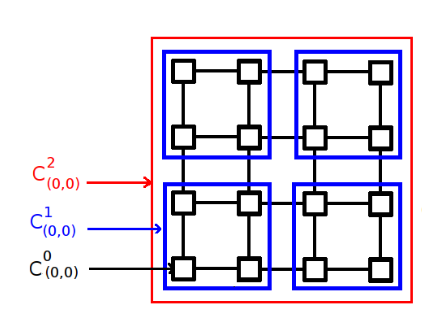
\includegraphics[scale=0.4]{dqdt-logical}
        \caption{Découpage de la plateforme}
        \label{fig:dqdt-logical}
      \end{subfigure}
      \begin{subfigure}[b]{0.4\textwidth}
        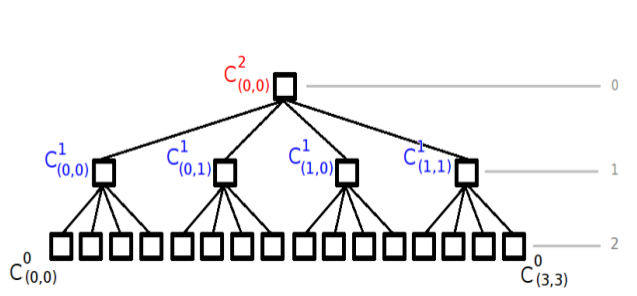
\includegraphics[scale=0.4]{dqdt-tree}
        \caption{Représentation du découpage}
        \label{fig:dqdt-tree}
      \end{subfigure}
      \caption{Construction de la DQDT~\citep{almaless2014universite}.}
    \end{figure}

    La DQDT, comme la plupart des composant noyaux d'ALMOS, repose sur le
    mécanisme de la mémoire virtuelle répartie entre les clusters. Si l'on passe
    ALMOS en mode multi-noyau, les serveurs de la DQDT ne peuvent plus
    communiquer grâce à la mémoire virtuelle. Ils sont obligés d'utiliser le
    passage de messages entre les noyaux.

    Notre but est donc de changer le schéma de communication de la DQDT en
    utilisant le passage de message.
